\chapter{Fisica Medica}

\begin{itemize}
	\item \textbf{CT (TAC in italiano)} tomografia assiale computerizzata
	\item \textbf{Risonanza Magnetica, MRI, fMRI}: array tridimensionali, volendo anche nel tempo, quindi 4-dimensionali.
	\item 
\end{itemize}

La conoscenza dei meccanismi fisici che generano il dato su cui lavoriamo è importante.\\
Le immagini mediche non sono semplici fotografie, ma sono immagini che contengono importanti informazioni sullo stato di salute del corpo umano.\\

\begin{figure}[ht]
	\centering
	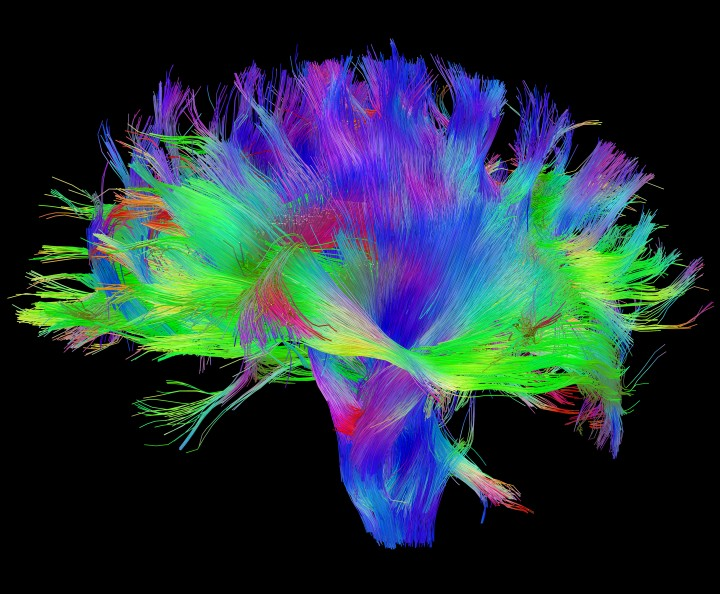
\includegraphics[width=0.6\linewidth]{figure_med/White-Matter-Fibers.jpg}
\end{figure}
\FloatBarrier

Le immagini mediche riflettono diverse proprietà fisiche del corpo umano. Esse sono formate dall'interazione tra radiazione/ultrasuoni con i tessuti/organi.\\


\subsection{Le principali modalità di imaging diagnostico}
Quando si parla di radiografia tipicamente ci si riferisce a immagini 2D.\\
Tomografia invece si rifersice a immagini 3D.\\


Lo sforzo moderno è quello di creare dispositivi multimodali, che investigano il corpo umano da diversi punti di vista. Acquisire informazioni complementari attraverso le diverse modalità contemporaneamente. Unendo le informazioni possiamo ottenere una diagnosi più accurata.\\
Ogni tecnica ha una specifica risoluzione spaziale, combinando le varie tecniche possiamo migliorarla.\\

\textbf{Medicina di precisione}: creare un trattamento specifico per ogni paziente. A contrapporsi ad un metodo basato su protocolli, come si fa attualmente nel nostro sistema sanitario.\\
Mettendo insieme tutte le informazioni sul paziente si può arrivare a delle diagnosi e a dei trattamente altamente personalizzati.\\
Sfida: come inegrare i dati che vengono da sorgenti diverse in maniera efficiente.\\

\subsection{Il ruolo dei computer nell'imaging medico}
Da sempre i computer hanno un ruolo fondamentale nell'imaging medico.\\
I dati \textit{raw} devono essere interpretati ed elaborati attraverso algoritmi di ricostruzione per poterli poi fornire al medico. Si usano algoritmi di denoising basati sull'intelligenza artificiale.\\



\begin{figure}[ht]
	\centering
	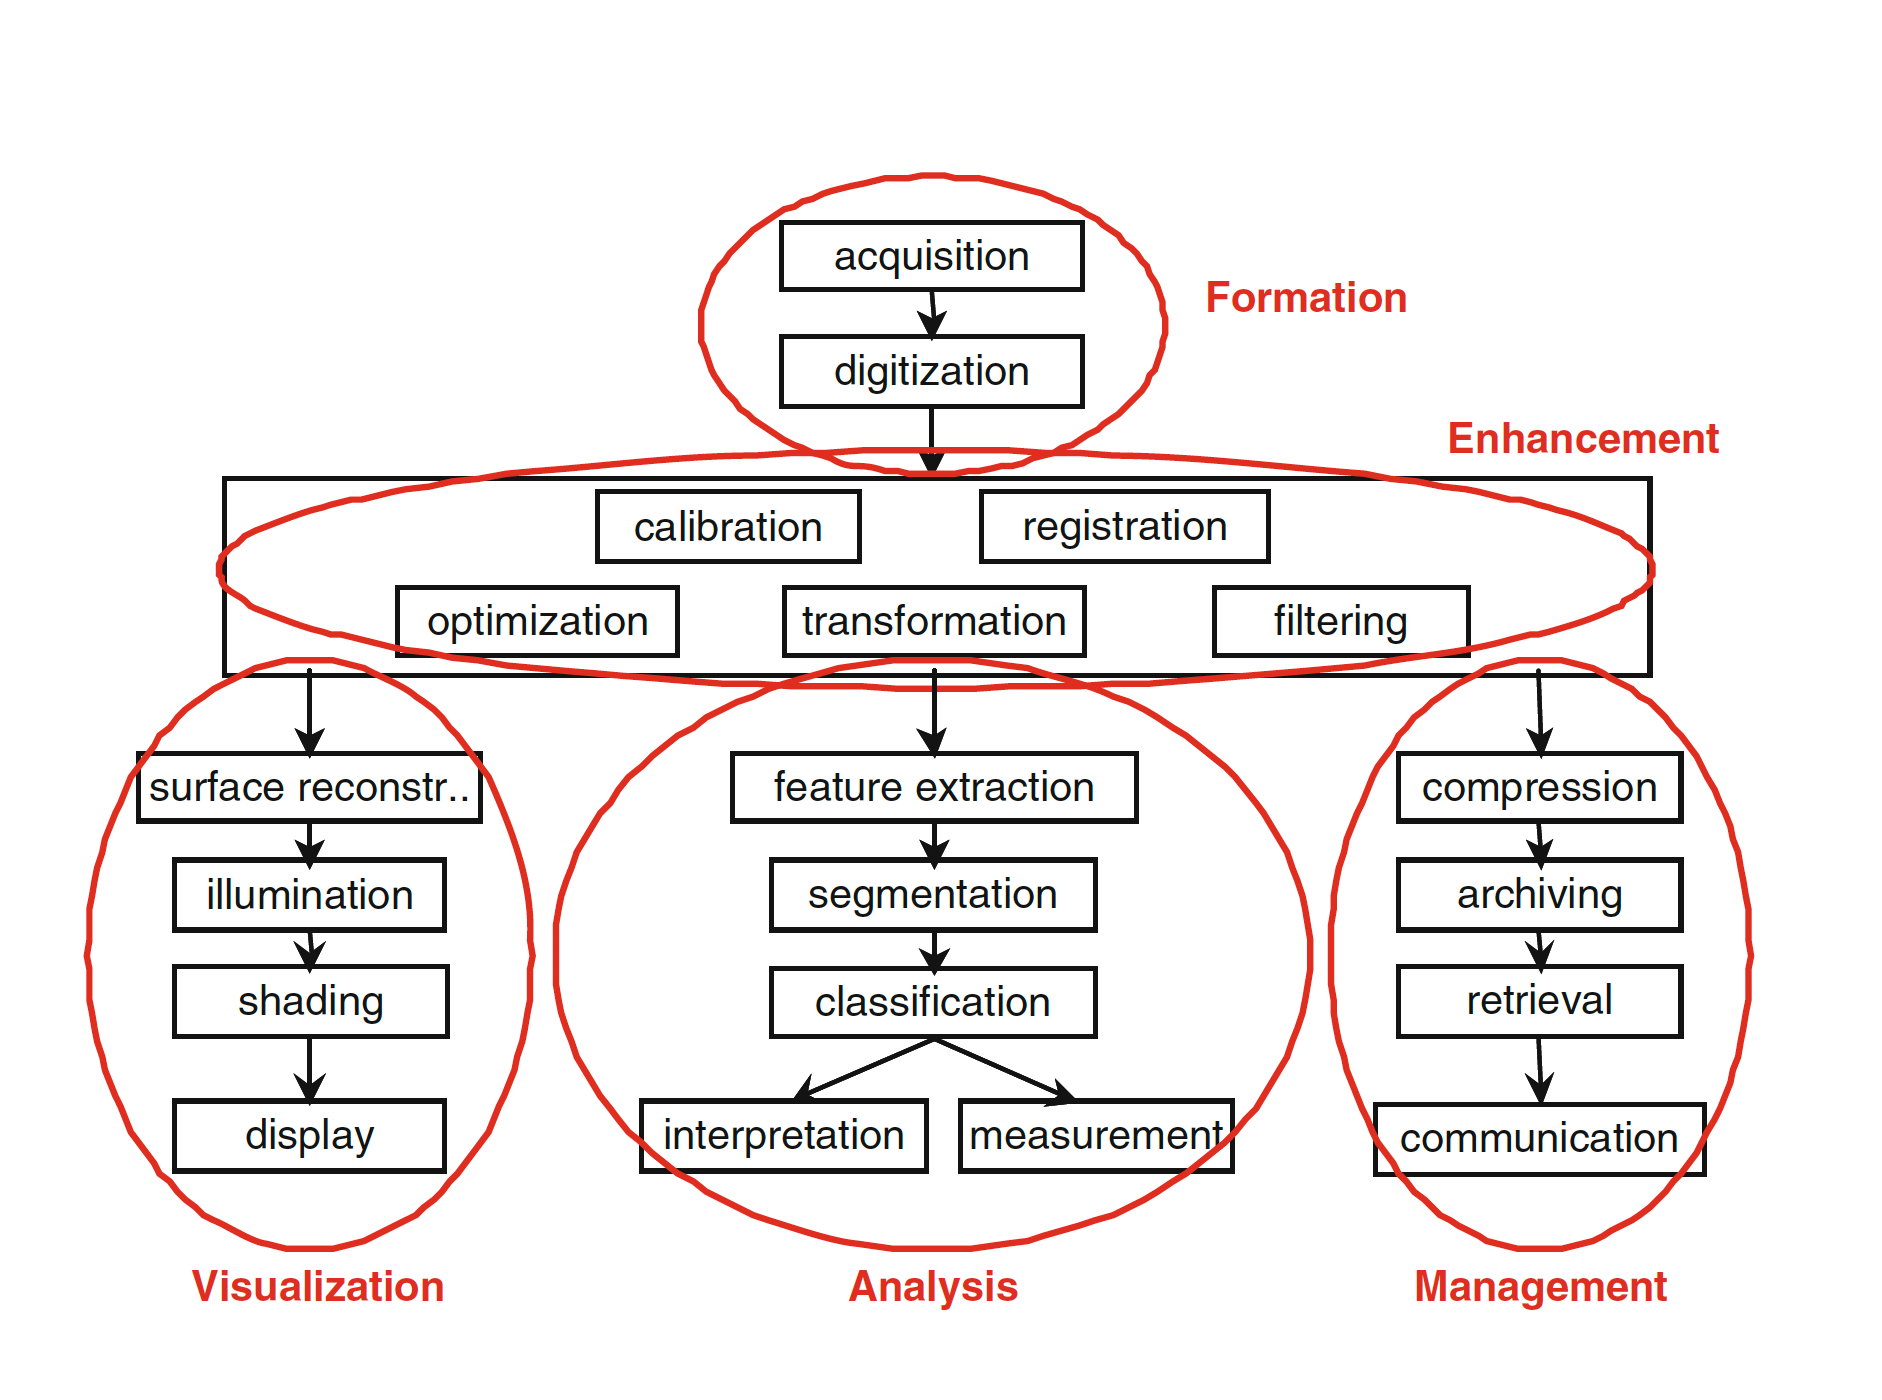
\includegraphics[width=1\linewidth]{figure_med/computers_med_img}
	\caption{Algorithms for
		information processing
		enter at many levels in
		the image formation
		pipeline}
\end{figure}
\FloatBarrier
In questo corso: a partire dall'immagine medica acquisita (già con valore diagnostico per un medico), possiamo lavorarci sopra per acquisire informazione. Ad esempio mettendo su degli algoritmi di classificazione.\\

\subsection{Biomedical image processing and analysis}

Il nostro obiettivo è identificare delle anomalie nelle immagini. Identificare lo stato di avanzamento di una certa lesione, per studiarne il tasso di crescita.\\
Vorremmo costruire uno strumento che sia il più robusto possibile ad una serie di variabilità a cui è esposta la lettura del medico, e che sia \textbf{riproducibile}, in modo da affiancare il medico nel processo decisionale.\\

The main objectives are:
\begin{itemize}
	\item To detect abnormalities in diagnostic images (lesions, etc.)
	\item To follow up pathological conditions (e.g. measuring the growth rate of lesions)
	\item To assess treatment efficacy
\end{itemize}


\subsection{Data dimensionality: 3D images}

Dal sinogramma lavoro con degli algoritmi di ricorstruzione, da cui poi posso ricavare delle immagini (a fette) che rappresentano l'anatomia del paziente..

(micronodulo polmonare)\\

\subsection{Volume display planes}
Una TAC del torace è un volume tridimensionale.\\

Medical images are usually displayed by anatomical planes.

\subsection{Data dimensionality: 3D and more…}

\begin{figure}[ht]
	\centering
	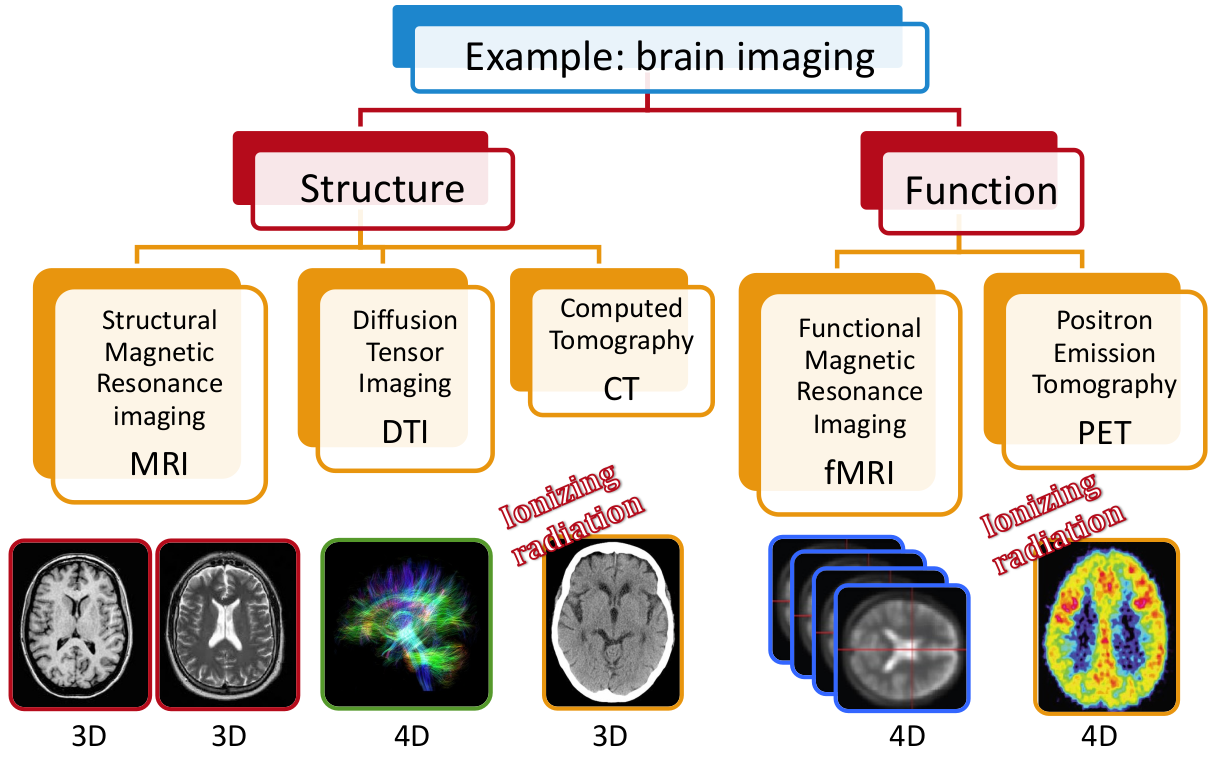
\includegraphics[width=1\linewidth]{figure_med/data_dim}
\end{figure}
\FloatBarrier

\subsection{Structural MRI $T_1$ -weighted images}

\subsection{Functional MRI (fMRI)}

\begin{itemize}
	\item BOLD Response: blood-oxygen-level-dependent (BOLD) contrast
	\item Typically, 1 volume per second (3x3x3mm$^3$ ) is
	acquired for 4-5 min
	\item Stimuli (visual, auditory, tactile, …) are
	administered to the subject during the scan
	\item Analysis of data time series to look for up-and-
	down signals that match the stimulus time
	series
\end{itemize}

\textbf{Functional connectivity}

\begin{itemize}
	\item Resting state rs-fMRI: study of temporal correlations between spatially remote neurophysiological events
\end{itemize}

\subsection{Data dimensionality: 2D/3D/4D/..nD images}

\begin{figure}[ht]
	\centering
	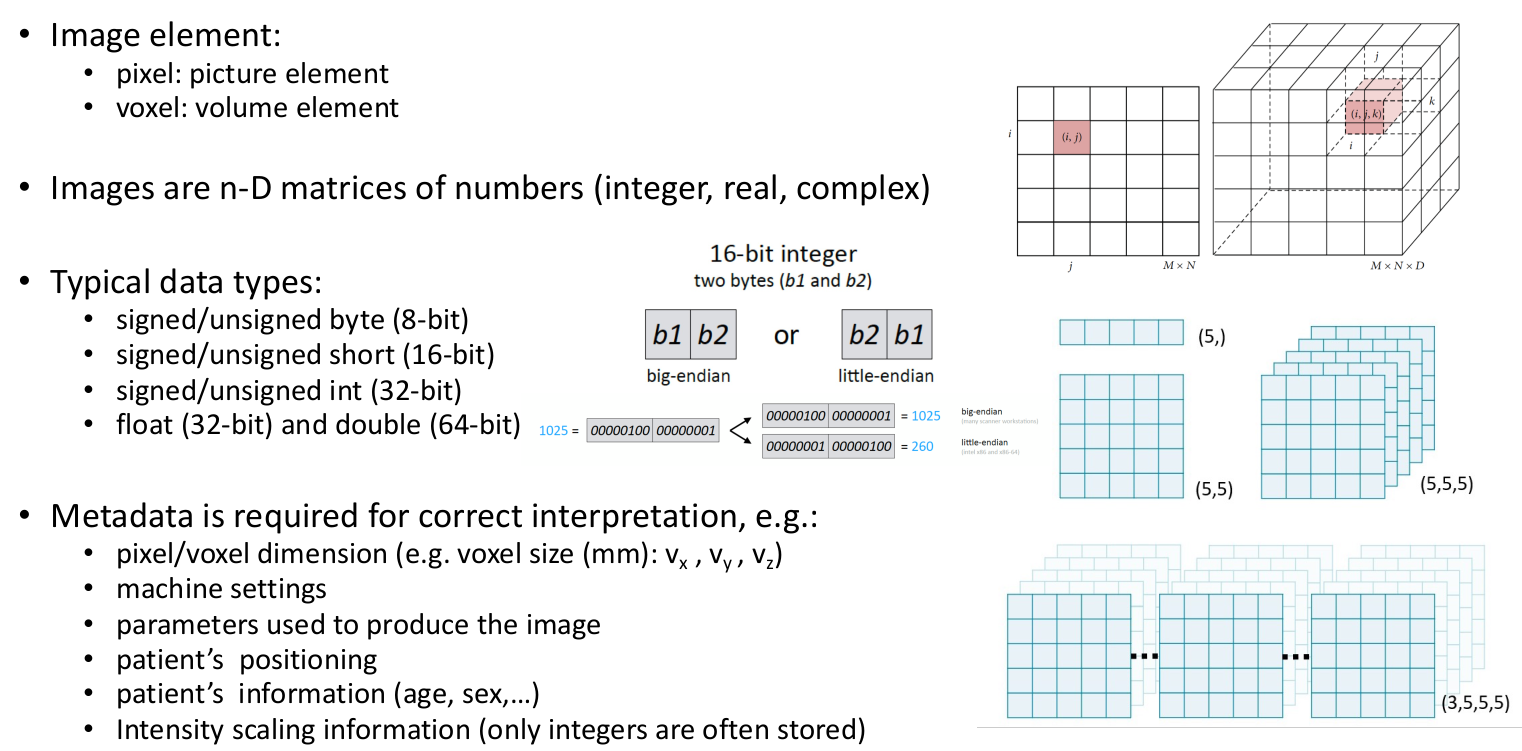
\includegraphics[width=1\linewidth]{figure_med/datadim}

\end{figure}
\FloatBarrier


L'immagine medica non è solo l'array n-dimensionale di dati. Ma deve contenere consistentemente tutte le informazioni neccassarie ad interpretare tali dati.

\subsection{Errors introduced by the analog to digital conversion}

\begin{figure}[ht]
	\centering
	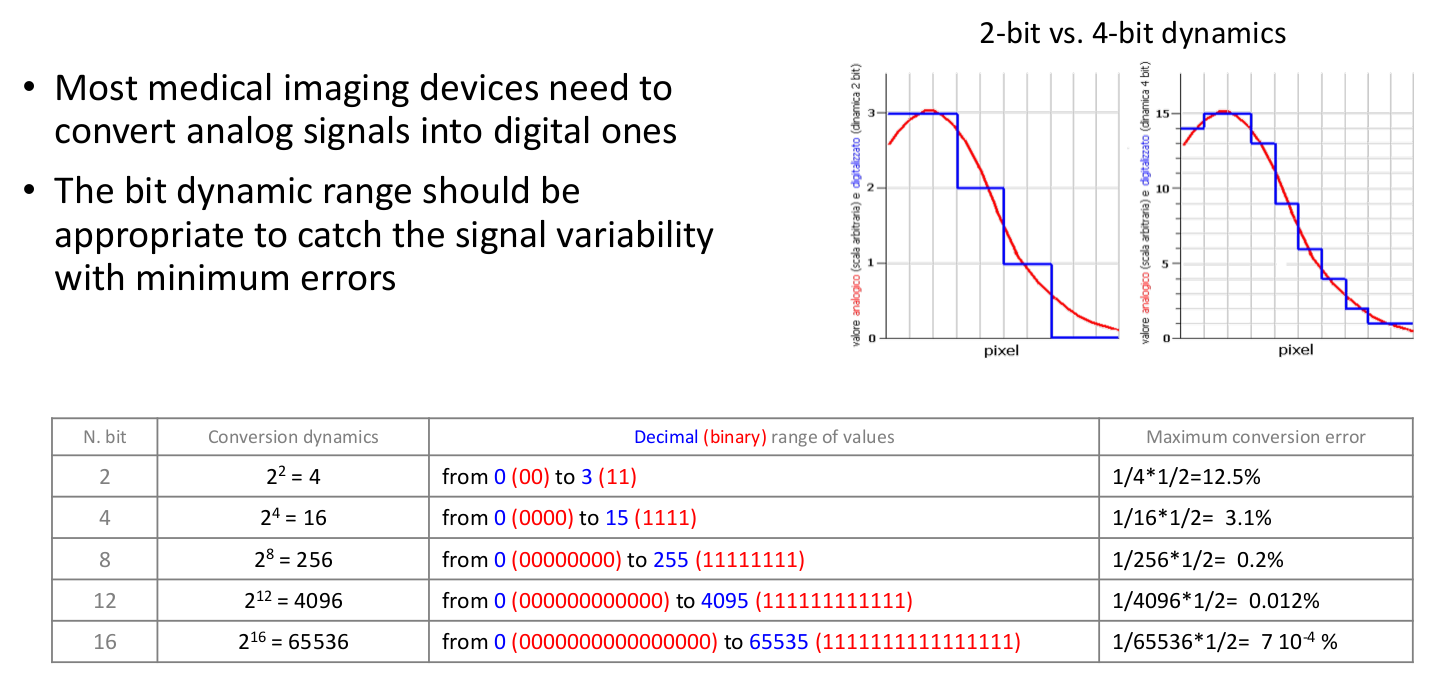
\includegraphics[width=0.9\linewidth]{figure_med/adc}
	
\end{figure}
\FloatBarrier


\subsection{Image representation with gray and color scales}


\begin{figure}[ht]
	\centering
	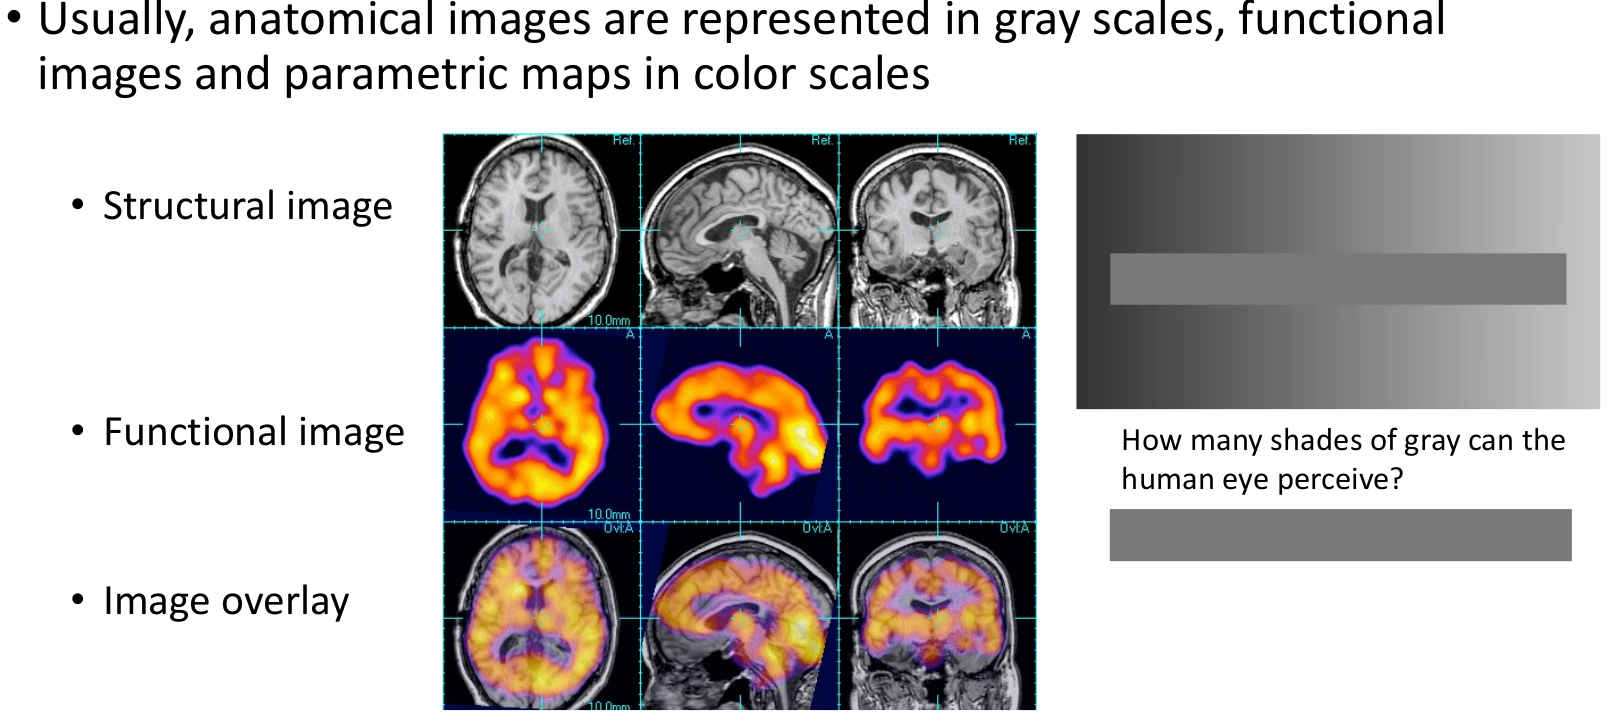
\includegraphics[width=0.9\linewidth]{figure_med/gray}
\end{figure}
\FloatBarrier

\subsection{Image windowing}

\begin{figure}[ht]
	\centering
	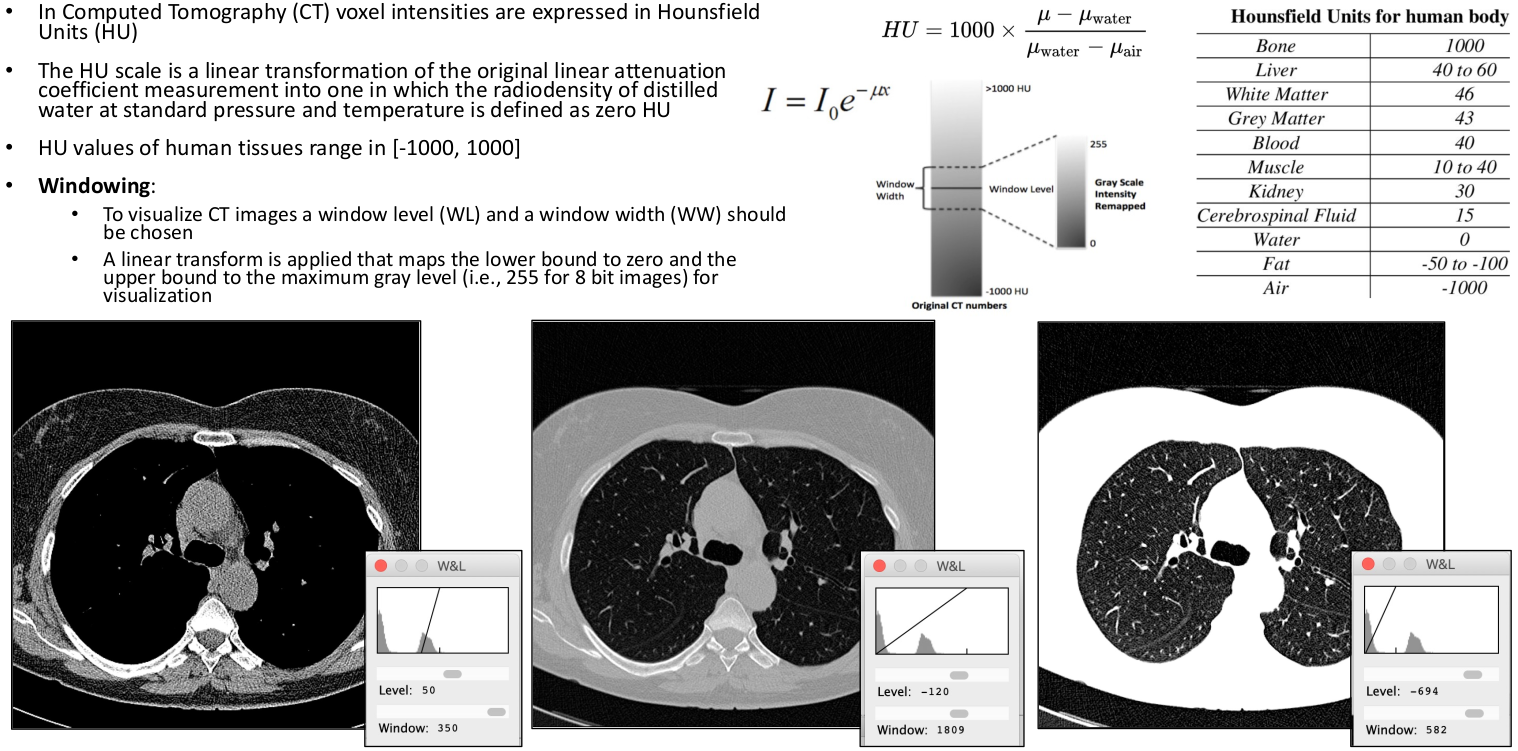
\includegraphics[width=0.9\linewidth]{figure_med/img_windowing}
\end{figure}
\FloatBarrier

\subsection{Look-up tables (LUTs)}

\subsection{Medical image file formats}



\subsection{The Neuroimaging Informatics Technology Initiative (NIfTI) file format}

\section{The General Data Protection Regulation (GDPR)}
